\section{Exercise 3}

In this section, we will show how using the lower cost technology
to implement a truth table, can result in some glitches and issues.
For this exercise, we were asked to simplify the truth Table on Table
\ref{3_1}.

\begin{table}[H]
\begin{centering}
\begin{tabular}{|c|c|c|c|}
\hline 
A & B & C & O\tabularnewline
\hline 
\hline 
0 & 0 & 0 & 0\tabularnewline
\hline 
0 & 0 & 1 & 1\tabularnewline
\hline 
0 & 1 & 0 & 1\tabularnewline
\hline 
0 & 1 & 1 & 1\tabularnewline
\hline 
1 & 0 & 0 & 0\tabularnewline
\hline 
1 & 0 & 1 & 1\tabularnewline
\hline 
1 & 1 & 0 & 0\tabularnewline
\hline 
1 & 1 & 1 & 0\tabularnewline
\hline 
\end{tabular}
\par\end{centering}
\caption{Truth Table}
\label{3_1}

\end{table}

When we express this in the form of the Karnaugh map, we'va got the
Figure \ref{3_2}. As we see there, if we do not take into account
the yellow minterm, there are two separate subsets of ones that can
represent the Table \ref{3_1}. However, as we know, because the two
subsets have no element in common, representing this truth tables
with just two minterms can cause glitches.

\begin{figure}[H]
\begin{centering}
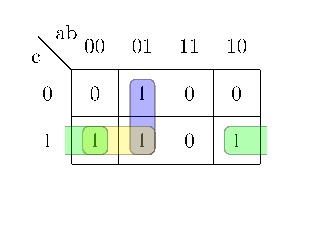
\includegraphics{images/Karnaugh}
\par\end{centering}
\caption{Karnaugh's Map}
\label{3_2}

\end{figure}

By implementing this wit NAND gates we've got the circuit shown on
Figure \ref{3_3}.

\begin{figure}[H]
\begin{centering}
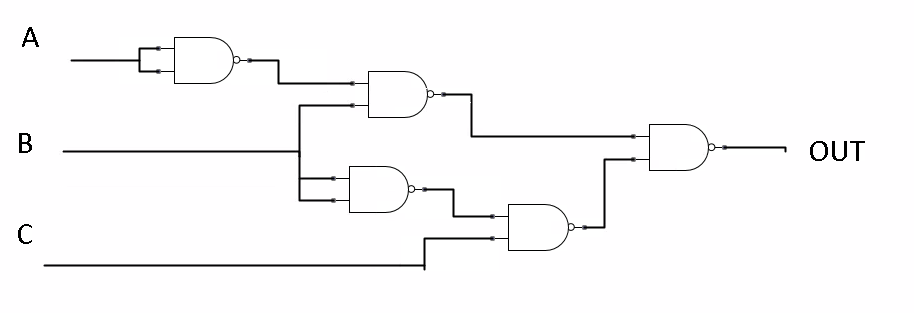
\includegraphics[scale=0.3]{images/CIRCUIT}
\par\end{centering}
\caption{NAND Circuit Implementation}
\label{3_3}

\end{figure}

Finally, when we tried to test the circuit shown, we noticed some
glitches of time less than 10 micorseconds, thes glitches are shown
on Figure \ref{3_4}.

\begin{figure}[H]
\begin{centering}
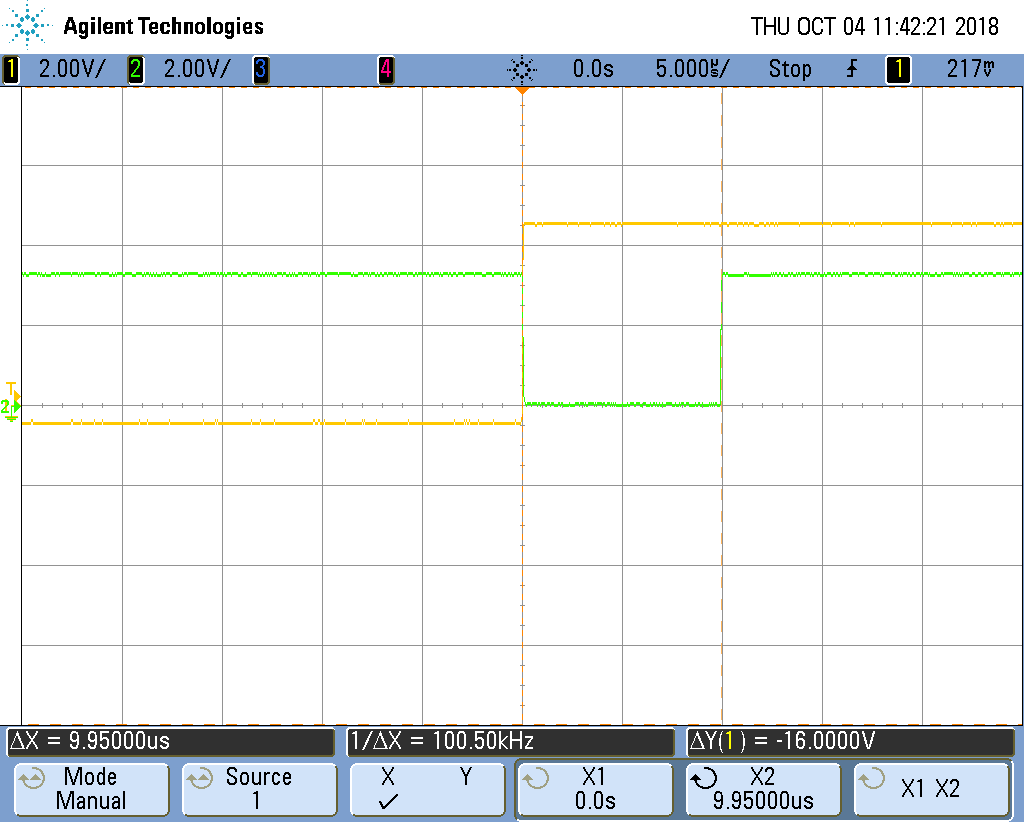
\includegraphics[scale=0.2]{images/e3}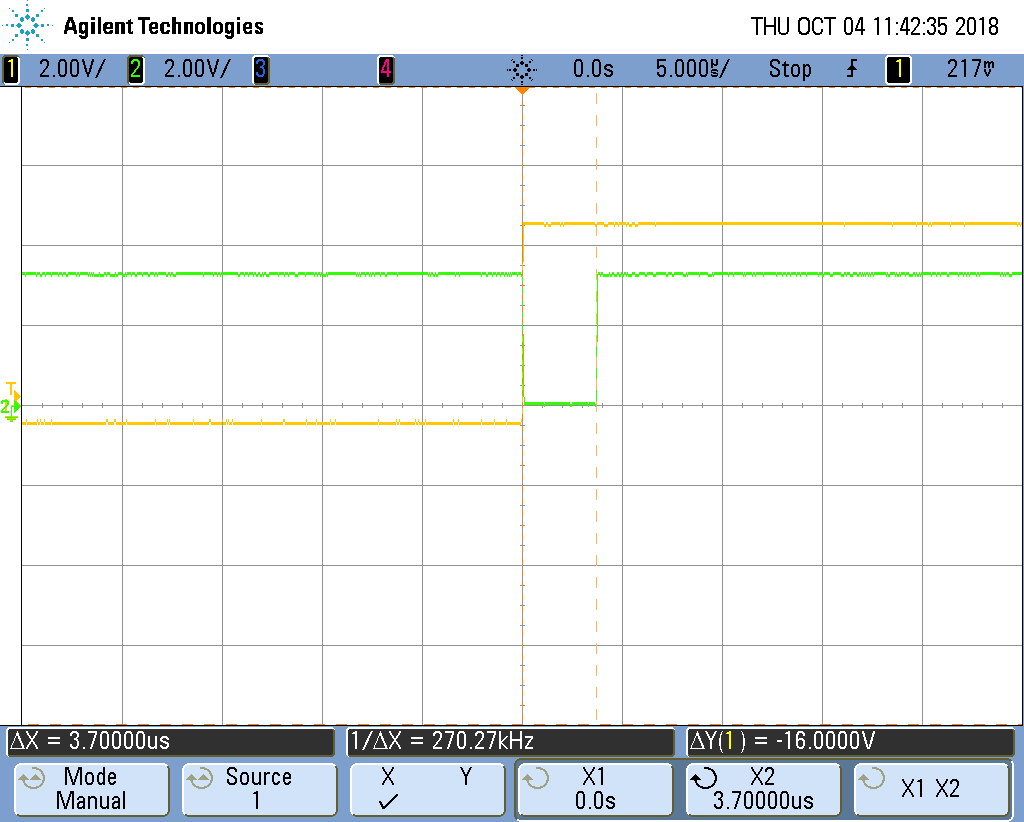
\includegraphics[scale=0.2]{images/e4}
\par\end{centering}
\caption{Glitches}
\label{3_4}

\end{figure}

This little negative peaks shouldn't be there since we were changing
from one positive state, to another positive state in both cases.
To resolve this, we only need to add a third minterm to the equation,
and this would be the yellow minterm on Figure \ref{3_2}.
